\documentclass[10pt,conference]{IEEEtran}
\IEEEoverridecommandlockouts
% The preceding line is only needed to identify funding in the first footnote. If that is unneeded, please comment it out.
\usepackage{cite}
\usepackage{amsmath,amssymb,amsfonts}
\usepackage{algorithmic}
\usepackage{graphicx}
\usepackage{textcomp}
\usepackage{xcolor}
\usepackage{url}
\newcommand{\todo}[1]{\textbf{\textcolor{red}{To do: #1}}}
\newcommand{\csp}[1]{\textbf{\textcolor{purple}{CSP: #1}}}
\newcommand{\ryo}[1]{\textbf{\textcolor{teal}{RY: #1}}}

\makeatletter
\newcommand{\linebreakand}{%
  \end{@IEEEauthorhalign}
  \hfill\mbox{}\par
  \mbox{}\hfill\begin{@IEEEauthorhalign}
}
\makeatother

\begin{document}

\title{OptoFlood: Controllable Flooding for NDN Producer Mobility}

\author{
    \IEEEauthorblockN{Yuting Wan}
    \IEEEauthorblockA{University of Glasgow\\
    yuting.wan@glasgow.ac.uk}
\and
    \IEEEauthorblockN{Ryo Yanagida}
    \IEEEauthorblockA{University of Glasgow\\
    ryo@htonl.net}
\and
    \IEEEauthorblockN{Paul Harvey}
    \IEEEauthorblockA{University of Glasgow\\
    paul.harvey@glasgow.ac.uk}
\linebreakand
    \IEEEauthorblockN{Jeremy Singer}
    \IEEEauthorblockA{University of Glasgow\\
    jeremy.singer@glasgow.ac.uk}
\and
    \IEEEauthorblockN{Colin Perkins}
    \IEEEauthorblockA{University of Glasgow\\
    csp@csperkins.org}
\and
    \IEEEauthorblockN{Leon Wong}
    \IEEEauthorblockA{Rakuten Mobile, Inc.\\
    leon.wong@rakuten.com}
}

\maketitle

\begin{abstract}

Producer mobility in systems that use Named Data Networking (NDN) protocols can lead to increased latency and packet loss due to problems with slow routing convergence. This affects applications, such as live video streaming and video conferencing, where even a brief interruption in packet delivery can degrade user experience. To address this, we propose \textit{OptoFlood}, a controllable flooding mechanism that supports Data and Interest packet delivery immediately following producer movement events, to rapidly establish temporary bidirectional communication paths. OptoFlood also accelerates global routing convergence through integration with the Named-data Link State Routing (NLSR) protocol. Our initial evaluation demonstrates that OptoFlood effectively reduces latency and packet loss, caused by producer mobility, while maintaining low network overhead.

\end{abstract}

\begin{IEEEkeywords}
Named Data Networking, Producer Mobility, NLSR, Routing
\end{IEEEkeywords}


\section{Introduction}
\label{sec:introduction}

% Paragraph 1: Motivation.
The use of Named Data Networking (NDN) protocols optimises the network for content delivery. Rather than indirect from name to location via the DNS, as done in the Internet today, NDN protocols make named-based routing, content delivery, and pervasive caching core services of the network.

% Paragraph 2: Specific problem.
A limitation of current NDN protocols, however, is that they don't effectively support producer mobility.  Each time a content producer moves, the network must quickly discover its new location and ensure continuous data delivery without introducing delays or packet loss. For applications such as live video streaming and video conferencing, even short interruptions can degrade the user experience and reliability. 
Prior work \cite{FIXME} has improved NDN behaviour in these scenarios, but performance still lags behind what is needed.
%Addressing producer mobility is therefore essential if NDN protocols are to see wide adoption.

%We consider the delay and packet loss caused by the slow routing convergence when NDN producers change their network attachment point. NDN producers must re-register their data prefix at each new network location and wait for global routing updates to propagate. During this convergence period, Interest packets may be misrouted or discarded due to outdated forwarding paths. Our baseline tests indicate that this can result in interruptions lasting several seconds, severely impacting latency-sensitive applications. In addition, repeated movements can exacerbate this issue, significantly affecting the overall performance of the network.

% Paragraph 3: Contributions.
In this paper, we introduce OptoFlood, a novel controlled flooding scheme that can establish temporary bidirectional communication paths to accelerate network convergence after producer mobility events. OptoFlood proactively manages controlled local flooding of both Data and Interest packets, enabling rapid recovery from disruptions caused by producer movements. 
%Producers initiate flooding by transmitting specially marked Data packets corresponding specifically to pending Interests received before the movement. These flooded packets are constrained to reach nodes that remain on, or near, the original forwarding path, thus rescuing Interests without waiting for global routing updates. Meanwhile, intermediate forwarders detecting invalidated forwarding entries perform Interest flooding with strictly limited propagation scopes, such as constrained hop counts, to efficiently locate the producer’s new attachment point. 
%Finally, OptoFlood 
It also integrates
%its flooding results 
with Named-data Link State Routing (NLSR), generating short-lived routing updates based on newly established temporary paths. This integration accelerates global routing convergence. Collectively, these mechanisms reduce latency and packet loss while maintaining low overhead in network resource usage.
Initial results show a \todo{XX}\% reduction in packet loss and a \todo{YY}\% reducing in convergence time from our approach (\S\ref{sec:evaluation}).

% Paragraph 4: Comparison to related work.
Compared to prior NDN mobility protocols, such as routing-based updates \cite{meddeb:2018:afirm}, Interest-based notification solutions \cite{auge:2016:map-me} or anchor-based tracing mechanisms \cite{zhang:2018:kite},
OptoFlood provides a more integrated and lightweight solution that leverages flooding as its primary mechanism for rapid path recovery and convergence. Unlike existing flooding solutions, our approach uses explicit controls, including hop limits and producer-side flood rate limits, to restrict the scope and duration of flooding, minimising unnecessary overhead. Additionally, by leveraging temporary bidirectional paths established via controlled flooding, OptoFlood accelerates global routing updates without relying on centralised anchor nodes, thereby avoiding single points of failure and reducing potential path inefficiencies.

% Paragraph 5: Roadmap.
We structure the remainder of this paper as follows. Section \ref{sec:problem} reviews the background of producer mobility problems in NDN, highlighting the limitations of traditional routing updates. Section \ref{sec:solution} presents the detailed design of OptoFlood, including the mechanisms for controlled flooding of Data and Interest packets, and the integration with NLSR to accelerate global convergence. Section \ref{sec:evaluation} describes our experimental setup and presents results that demonstrate the effectiveness of our approach. 
We discuss related work in Section \ref{sec:related}.
Finally, Section \ref{sec:conclusion} concludes the paper and briefly discusses potential directions for future enhancements of the OptoFlood approach.

% ==============================================================================
\section{Producer Mobility in NDN}
\label{sec:problem}

NDN shifts from a host-centric to a data-centric model, where content is identified by names rather than addresses. In NDN, communication relies on two core packet types: Interest Packets, sent by consumers to request data by specifying the content name, and Data Packets, returned by producers containing the requested content and related metadata. Both packet types follow a concise Type-Length-Value (TLV) encoding, enabling efficient processing and extendability.

NDN packet forwarders maintain a Content Store that caches Data packets; a Pending Interest Table (PIT) that records forwarded Interest packets awaiting the corresponding Data packets, ensuring accurate reverse path forwarding; and a Forwarding Information Base (FIB) that guides Interest packet forwarding.
When an Interest arrives at a forwarder, it checks the Content Store and returns the cached Data, if it is available. Otherwise, the PIT is checked to aggregate Interests and, if the Interest is new, it is forwarded based on the FIB. Figure~\ref{fig:NDN Packets Processing Flow} illustrates packet forwarding.

\begin{figure}[t]
    \centering
    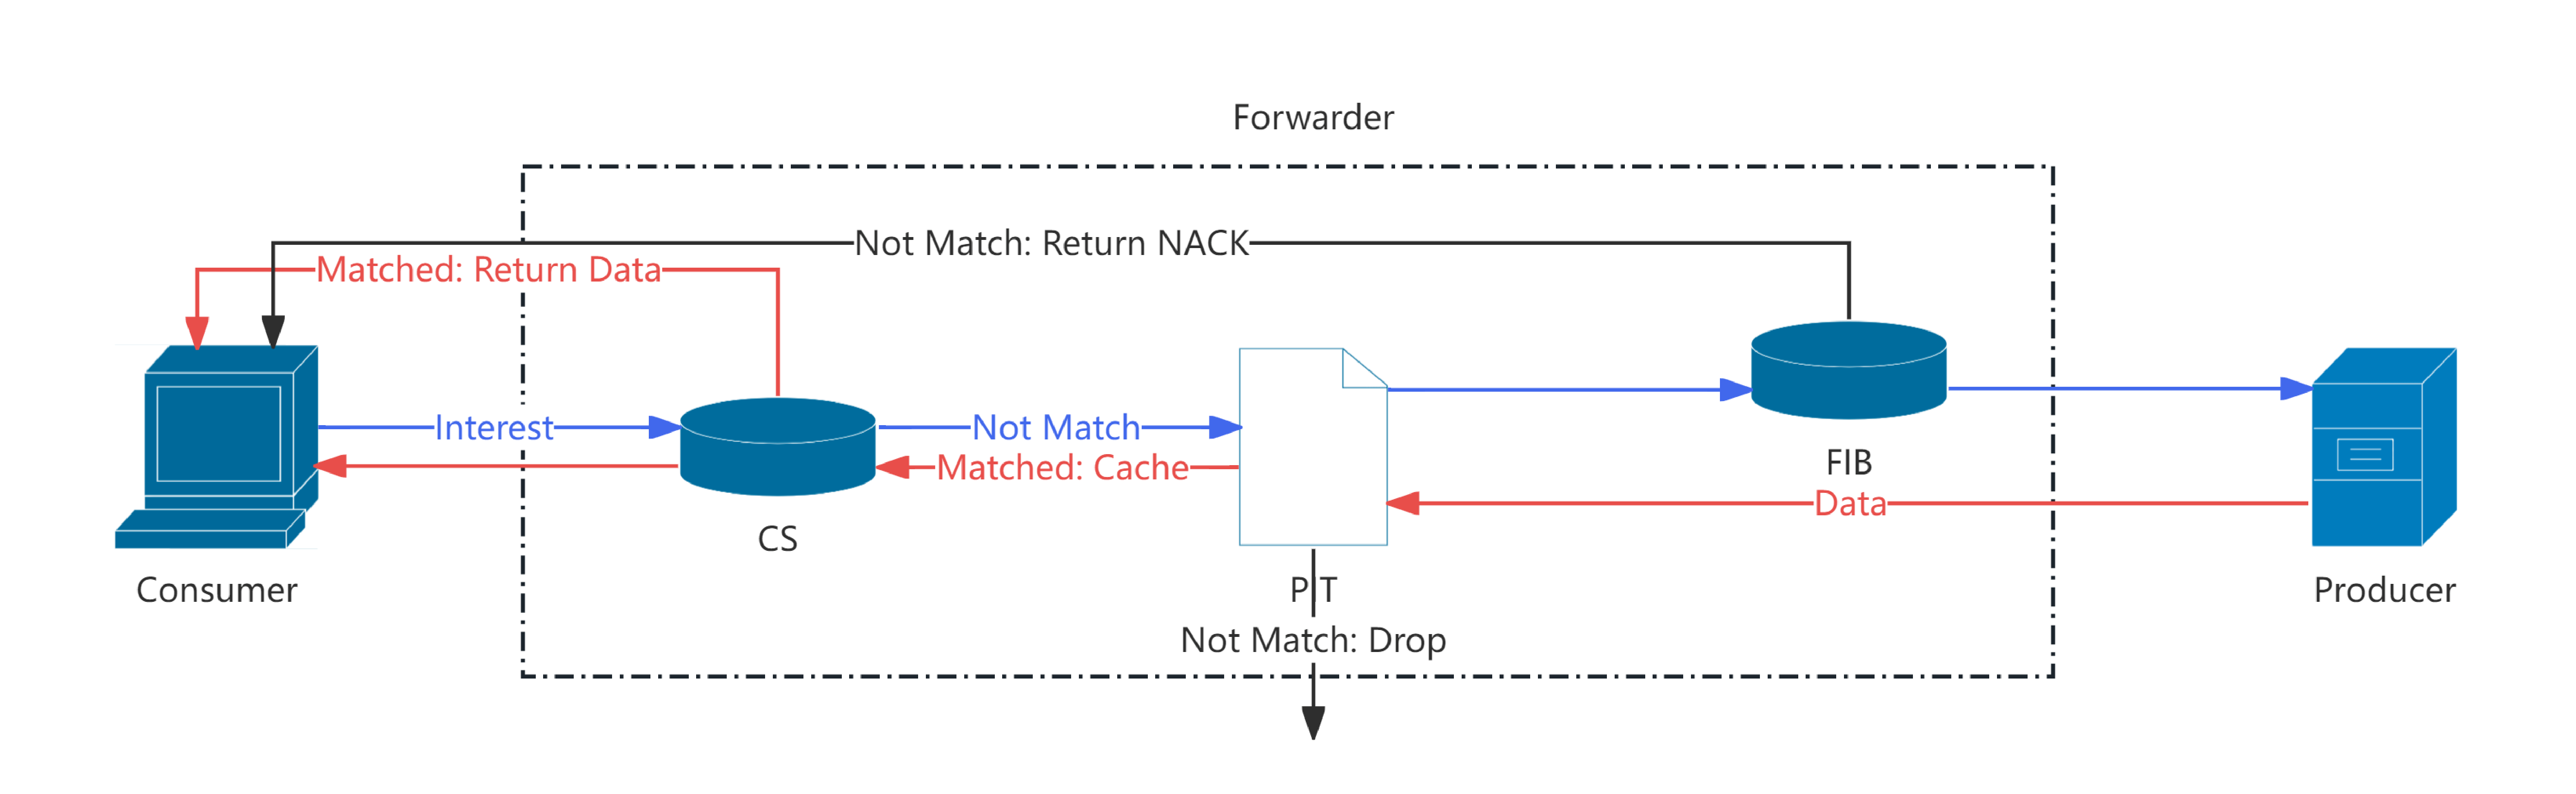
\includegraphics[width=1\linewidth]{NDN Packets Processing Flow.pdf}
    \caption{NDN Packets Processing Flow \csp{Update to make readable in single column form}}
    \label{fig:NDN Packets Processing Flow}
\end{figure}

The Named-Data Link State Routing protocol (NLSR) disseminates routing information via Link State Advertisements (LSAs) that carry link status and available data prefix information that are used to populate the FIB. NLSR adapts to network changes, such as node failures, new node attachments, or topology changes via periodic updates.

\begin{figure}[t]
    \centering
    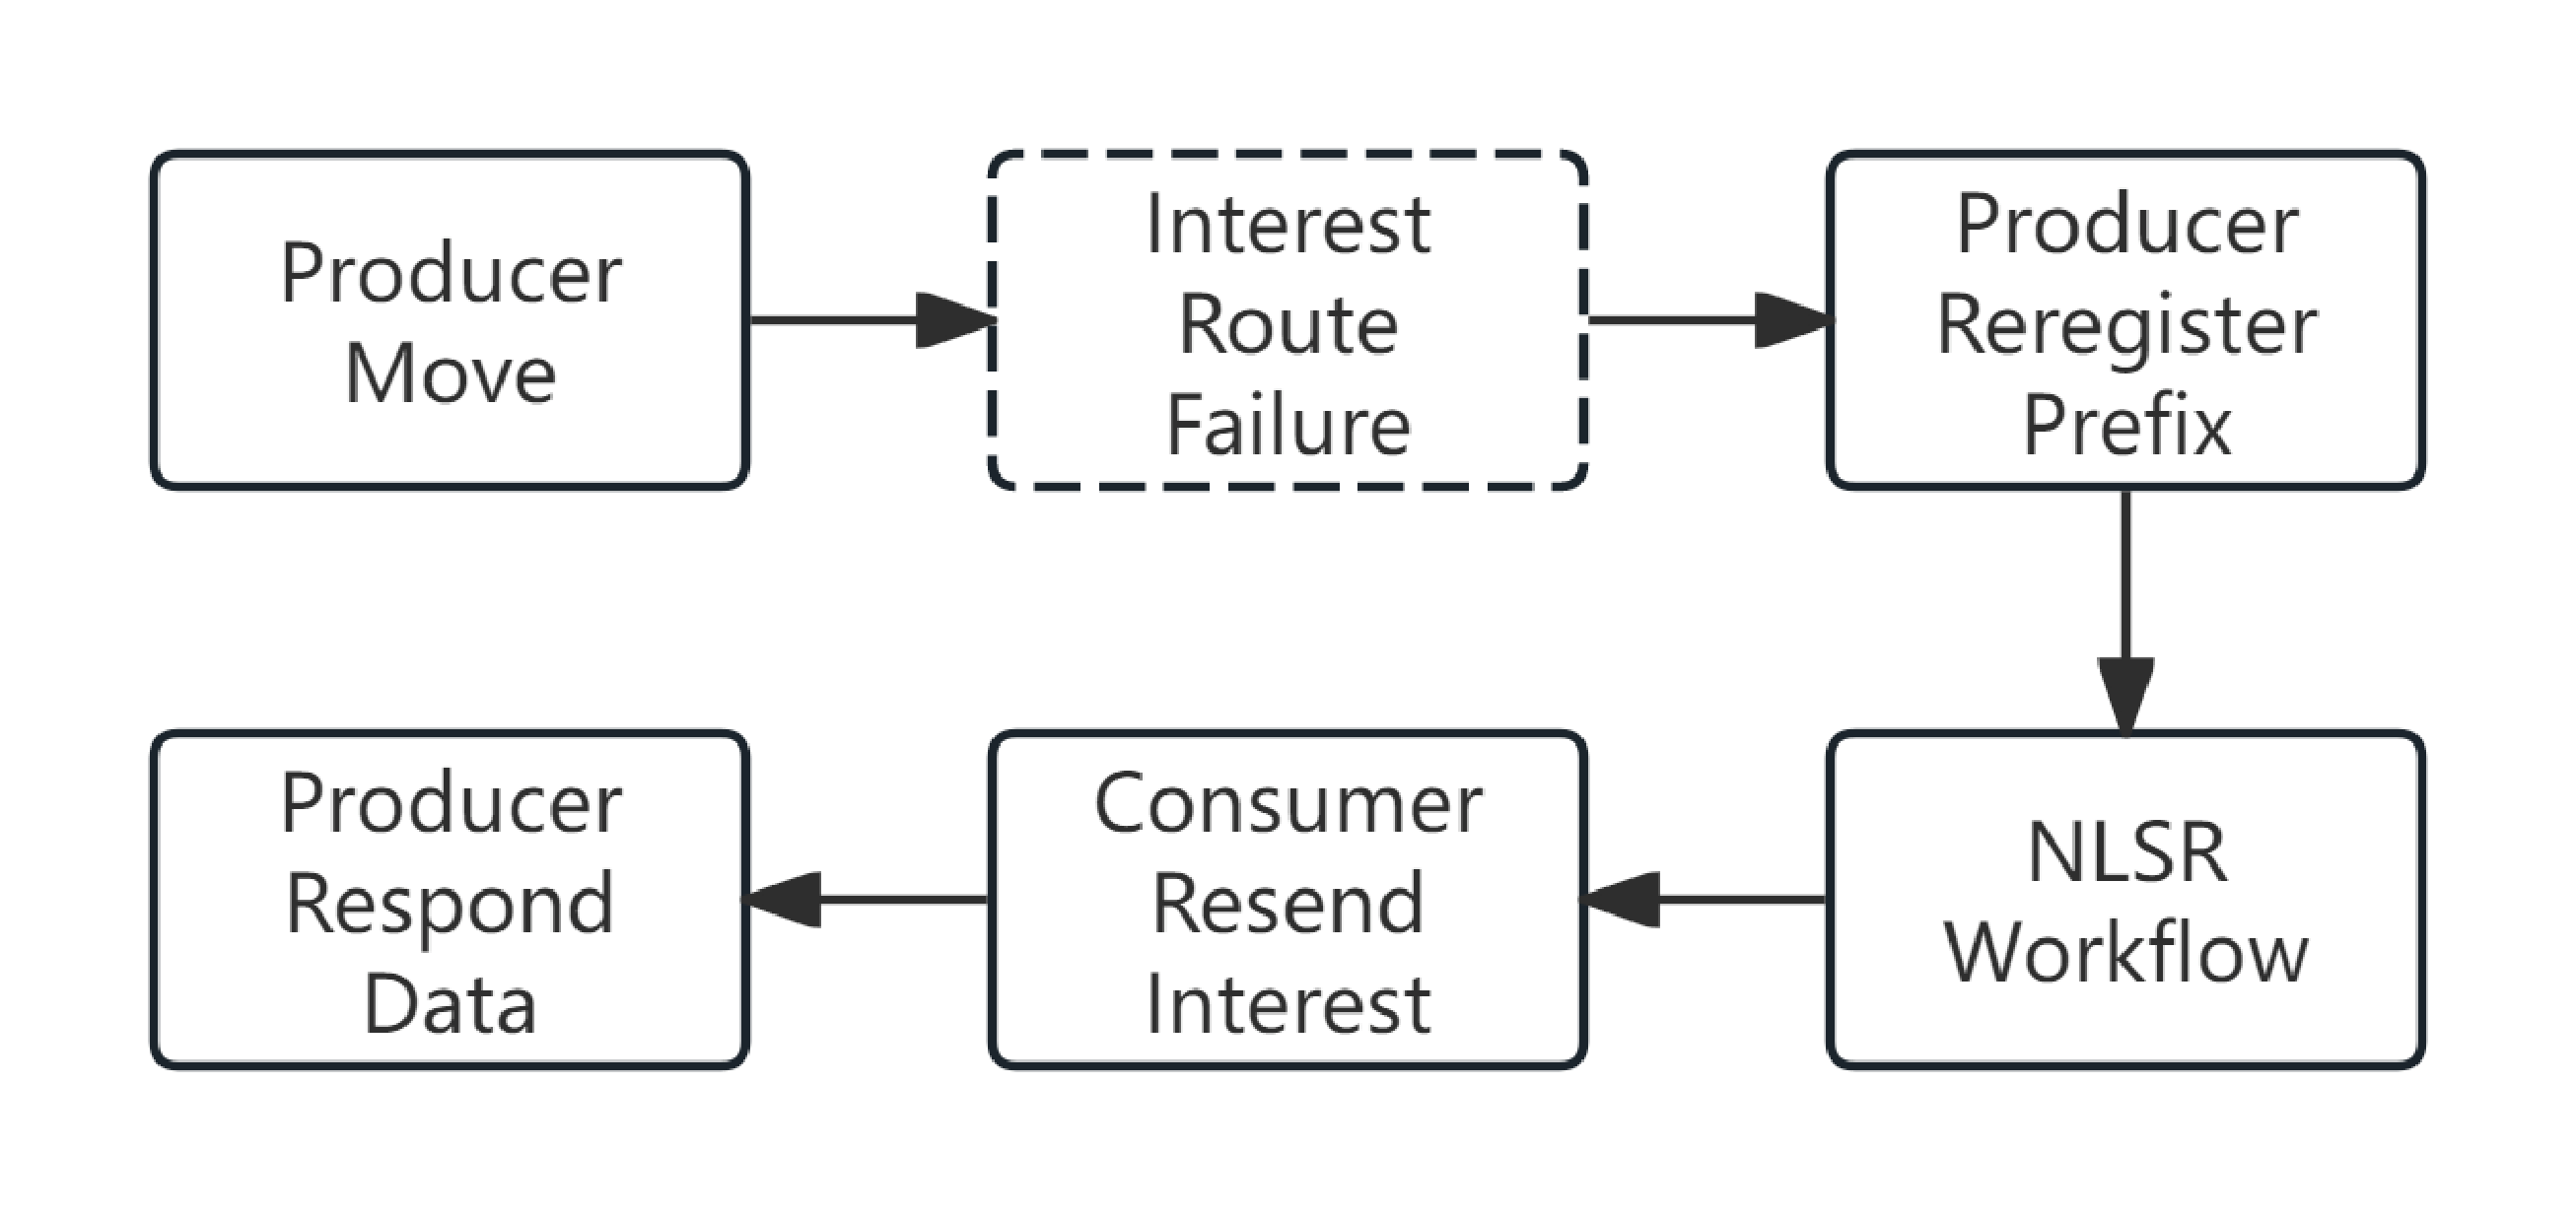
\includegraphics[width=1\linewidth]{NDN Producer Mobility Problem.pdf}
    \caption{NDN Producer Mobility Problem. \csp{To illustrate the problem, the figure should show the topology with packets being misdirected somehow; the current figure doesn't help.}}
    \label{fig:NDN Producer Mobility Problem}
\end{figure}

Producer mobility in NDN poses significant challenges, especially in dynamic network environments. Each time a producer moves, it must re-register its data prefix so that NLSR can propagate the updated routing information across the network. However, routing convergence through NLSR is inherently slow due to periodic dissemination of the LSAs and gradual propagation of routing updates (Figure~\ref{fig:NDN Producer Mobility Problem}). \csp{Does NLSR not send triggered updates when topology changes?}
This results in the following:
\begin{itemize}
\item \textbf{Increased Latency:} When a producer changes its attachment point, its associated data prefixes must be re-advertised, initiating routing updates starting from the directly connected forwarder. These updates must propagate throughout the entire network before Interest Packets can be delivered to the producer at its new location. During this convergence period, consumers experience significant communication interruptions, often lasting several seconds or longer \cite{FIXME}. In scenarios requiring low latency, such as live video streaming or real-time conferencing, even brief interruptions degrade the user experience \cite{FIXME} and severely limit NDN's practical utility.

\item \textbf{Packet Loss:} During producer relocation and the subsequent routing convergence process, Interest packets arriving at the producer's previous attachment point are unable to reach the new location, causing these packets to expire and be discarded. Additionally, data packets responding to interest received prior to relocation may be stranded at nodes lacking proper PIT entries, as the reverse paths have been invalidated. Without a valid return path, these Data packets remain undeliverable until their lifetimes expire, leading to further packet loss and negatively affecting communication reliability.

\item \textbf{Increased Network Resource Usage:} The inefficiencies introduced by latency and packet loss also result in increased retransmissions of interest packets \cite{FIXME}. These retransmissions consume additional bandwidth and processing resources across the network, potentially impacting overall network performance and affecting other communications.

\end{itemize}

These problems highlight the limitations of traditional routing-based approaches, such as NLSR, in handling frequent producer mobility. Addressing these issues effectively requires specialised mechanisms that can rapidly establish temporary communication paths without waiting for global routing convergence.

\csp{This section would benefit from some simulation results to show the extent of the problem. Space constraints may prevent us from including these.}

% ==============================================================================
\section{Controllable Flooding for NDN Mobility} 
\label{sec:solution}

To address the challenges of producer mobility in NDN, particularly in latency-sensitive applications such as video conferencing or live streaming, we propose \textit{OptoFlood}, a novel controllable flooding mechanism. OptoFlood rapidly establishes temporary bidirectional communication paths following producer movements and leverages these paths to accelerate global routing convergence.
OptoFlood also selectively incorporates beneficial elements from existing mobility solutions such as scoped flooding, inspired by MAP-Me \cite{FIXME}, and trace-guided forwarding from KITE \cite{FIXME} to further improve efficiency and performance.

\csp{Need a diagram showing the operation of the flooding, that the following can refer to.}

\subsection{Producer Mobility Detection and Data Packet Flooding}
\label{sec:solution:data-flooding}

When moving to a new Point of Attachment (PoA), the producer immediately initiates controlled flooding of Data packets corresponding to any Interest packets it had received prior to the handover, but to which it had not yet responded. These Data packets are marked in their MetaInfo TLV with:
\begin{itemize}
\item \textbf{MobilityFlag}: indicates mobility-related flooding.
\item \textbf{Flood-ID}: unique identifier for deduplication.
\item \textbf{NewFaceSeq}: sequence number that ensures consistency.
\item \textbf{Trace-Hint}: lightweight breadcrumb of recent PoAs (inspired by KITE~\cite{zhang:2018:kite}) for guided flooding.
\end{itemize}

These flooded Data packets preferentially follow existing valid FIB entries. If no valid FIB entry exists, the packets fall back to scoped blind flooding limited by a conservative maximum HopLimit of three hops, restricting propagation within typical local access and aggregation networks. The goal of this flooding is to reach nodes maintaining valid Pending Interest Table (PIT) entries, thus promptly rescuing pending Interests.

\subsection{Interest Flooding Triggered by Forwarder FIB Invalidation}
\label{sec:solution:interest-flooding}

Forwarders adjacent to the previous PoA detect invalid FIB entries upon receiving Interest packets without available next hops. These forwarders initiate controlled flooding of only the initial batch of Interests directly impacted by producer relocation. Flooding is triggered explicitly after the forwarder observes explicit invalidation signals, such as receiving NACK packets or reaching a predefined consecutive Interest failure threshold.
The Interest flooding strategy involves:
\begin{itemize}
\item \textbf{Prioritised Forward}: Forwarders first attempt to forward Interests via existing valid FIB entries towards last known PoAs, guided by \textit{Trace-Hints} embedded within Interest packets.
\item \textbf{Scoped Blind Flooding}: In the absence of valid FIB entries, forwarders employ scoped blind flooding inspired by the local discovery mechanism of MAP-Me~\cite{auge:2016:map-me}, restricting packet propagation by using a conservative HopLimit (typically set to 3).
\end{itemize}

This controlled flooding efficiently discovers the producer's new location, minimising unnecessary network load.

\subsection{Temporary Bidirectional Path Establishment}
\label{sec:solution:bidir}

OptoFlood leverages the coordinated flooding of Interest and Data packets to establish robust temporary bidirectional paths. When flooded Interests reach the relocated producer, returning Data packets carry updated \textit{NewFaceSeq} and \textit{Flood-ID}. Forwarders receiving these Data packets establish or update a separate Temporary FIB (TFIB), distinct from the standard FIB, specifically designed to handle transient mobility-related paths.
\csp{Why a temporary FIB rather than state in the existing FIB?}

The TFIB entries maintain temporary forwarding states with a brief TTL (approximately one second \csp{why this value?}), a duration selected to quickly remove transient forwarding states after global routing convergence, thereby minimising memory and state overhead.

Flooded Data packets returning downstream primarily follow existing PIT entries towards consumers. If PIT entries have expired, the packets return to TFIB entries, ensuring reliable downstream connectivity.

Thus, the combination of controlled Interest and Data packet flooding rapidly and effectively bridges temporary communication gaps caused by producer mobility, ensuring minimal disruption for latency-sensitive applications.


\subsection{Accelerated Network Convergence}
\label{sec:solution:convergence}

OptoFlood uniquely integrates temporary flooding-based paths with global routing convergence via Named-data Link State Routing (NLSR) \cite{}. Whenever a forwarder establishes a TFIB entry due to successful flooding, it immediately generates and disseminates a short-lived \csp{What is meant by ``short-lived''?} Fast-LSA, which includes the \textit{NewFaceSeq} and the face information learnt from the flood results. The Fast-LSAs are generated only upon TFIB creation, rather than upon other forms of mobility detection. This is because TFIB entries explicitly confirm new valid forwarding paths identified by successful flooding. In contrast, other unverified mobility detections could introduce erroneous information or routing instability. This Fast-LSA rapidly propagates among neighbouring nodes, typically within milliseconds, significantly accelerating local route convergence. Regular periodic LSAs subsequently replace these Fast-LSAs, allowing TFIB entries to gracefully expire. This approach accelerates global convergence without requiring core NLSR modifications.

\subsection{Security and Flooding Control}

To help mitigate the security risks associated with flooding, OptoFlood uses three complementary mechanisms.

First, NDN Data packets contain digital signatures that authenticate static packet fields such as names and content, protecting packet integrity and authenticity from intermediate node manipulation. Dynamic fields like \textit{MobilityFlag} (changed upon PIT match) and \textit{HopLimit} (decremented hop-by-hop) cannot be authenticated by signatures, as a legitimate intermediate modification occurs. Thus, signatures provide baseline authenticity rather than complete tamper protection for dynamic fields.

Second, a global maximum HopLimit threshold (\S\ref{sec:solution:data-flooding}) is enforced throughout the network, derived from the typical hop distances of the mobile network between PoAs. This prevents malicious producers from initiating flood attacks with excessive hop counts, ensuring that flooding remains confined to local access or aggregation layers.

Third, strict flood rate limits per producer (60-100 packets / second) prevent resource exhaustion, effectively protecting against Denial-of-Service (DoS) attacks by restricting flood volumes within realistic network capacity limits.

Together, these mechanisms maintain a robust security posture without significantly increasing complexity or overhead.

% ==============================================================================
\section{Evaluation}
\label{sec:evaluation}

We evaluate OptoFlood in micromobility \ryo{what is micromobility? can we just say mobility?} scenarios with real-time video, representing common conferencing and live streaming applications.

% ------------------------------------------------------------------------------
\subsection{Methodology}

We focus on campus micro-mobility with real-time video: a smartphone user walks across a campus network, with the connection handing over between nearby Points of Attachment (PoAs) under the same distribution domain while the video stream remains active. This is a common, real-world, scenario that must work effectively with NDN and that is sensitive to latency, packet loss, and transient routing disruption.

% In this local setting, the new attachment is typically within two to three hops of the previous path. OptoFlood scopes propagation accordingly (small hop limits) and writes short-lived temporary forwarding entries to form a transient bidirectional path; the confirmed path information is then used to speed up convergence of the routing plane.
% 
% We focus on real-time video transmission as the primary application scenario due to its high sensitivity to latency, packet loss, and transient routing disruptions. Such conditions are typical in mobile video conferencing, live streaming from smartphones, or moving between WiFi hotspots, where even brief interruptions can significantly impact user experience.

% - - - - - - - - - - - - - - - - - - - - - - - - - - - - - - - - - - - - - - -
\subsubsection{Producer Application}
We implement a typical NDN video producer with our mobility extensions.
Generated video Data packets have a threshness period of 10 seconds, permitting caching but preventing stale data from clogging the network, and carry a payload of synthetic data matching the size and timing of video content. Packets are digitally signed to ensure integrity and security.
Content prefixes are advertised via NLSR in the usual manner, with the extensions discussed in Section \ref{sec:solution}.

% The producer application generates Data packets in response to Interests and incorporates necessary mobility indications to enable OptoFlood’s controlled flooding and route convergence acceleration. The application itself remains primarily focused on standard data processing tasks, with mobility handled through simple packet markings.
% 
% \textbf{Prefix Registration:}
% The producer advertises its data prefix (e.g., \texttt{/example/testApp}) to the network using standard NLSR commands (e.g., \texttt{nlsrc advertise}), enabling correct Interest forwarding.
% 
% \textbf{Interest Packet Processing:}
% Upon receiving an Interest packet matching its prefix, the producer promptly generates and returns the corresponding Data packet, setting a freshness period of 10 seconds to ensure timeliness aligned with typical video application requirements.
% 
% \textbf{Data Content Generation and Signing:}
% Data payloads in the current experiment use placeholder strings (e.g. "Hello, world!") to simulate real-time data characteristics. Although not employing actual video content, these payloads maintain consistent sizes to reflect realistic video packet profiles. Generated Data packets are digitally signed using the default keychain, ensuring integrity and security.
% 
% \textbf{Mobility Detection and Flooding Preparation:}
On detecting changes in its network attachment point, the producer marks pending Data packets with a \texttt{MobilityFlag} within the MetaInfo TLV.of the packet. Additionally, each marked packet includes a unique Flood-ID (for duplicate detection), a sequence number (ensuring correct ordering and consistency), and a trace-hint (a lightweight path indicator derived from recent attachment points, guiding packet direction during flooding). 
% These markings prepare Data packets for controlled flooding, rescuing pending Interests affected by mobility events.
% 
% \textbf{Controlled Data Packet Flooding:}
As described in Section \ref{sec:solution}, marked Data packets are flooded in a constrained manner.
% starting from the new PoA. Flooding prioritises forwarding based on existing FIB entries whenever possible, resorting to limited, scoped flooding (1–2 hops) only when no valid FIB entries exist. Controlled flooding employs hop-limit restrictions and trace-hints to ensure efficient propagation toward nodes on the previous forwarding paths.

%\textbf{Error Handling:}
%Prefix registration failures result in error messages and termination of forwarding operations to prevent unnecessary resource usage. Mobility events and packet marking actions are logged internally but do not disrupt application operation, as forwarders handle the flooding process transparently.
% 
% This design ensures real-time responsiveness, relying on OptoFlood to manage producer mobility without placing undue complexity on the application itself.


% - - - - - - - - - - - - - - - - - - - - - - - - - - - - - - - - - - - - - - -
\subsubsection{Consumer Application}

\csp{This is too long: one paragraph only}

The consumer application continuously issues Interest packets and processes received Data packets to simulate realistic, real-time video stream handling. Maintains a straightforward NDN-based operation without explicit mobility awareness, relying instead on the underlying network mechanisms provided by OptoFlood.

\textbf{Automatic Data Requests:}
The consumer sends Interests with a predefined name prefix (e.g., \texttt{/example/livestream/}) appended by sequential version numbers to uniquely identify each data chunk. The interest packets are marked as "must be fresh" and set with a lifetime of 6 seconds to ensure timely delivery, aligning with typical real-time video requirements (simulating 30 frames per second).

\textbf{Request Frequency:}
The application generates Interest packets at intervals of 33 milliseconds, simulating the typical frame rate of a real-time video stream.\ryo{which is? (use fps for frame-rate)} This frequency ensures realistic load conditions without overwhelming network resources.

\textbf{Management of Unresponsive Interests:}
Timed-out Interests are placed into a First-In-First-Out (FIFO) queue for retransmission at a controlled, lower frequency of once per second. \ryo{wouldn't the application want to be more aggressive?} Retransmissions are triggered by Interest timeouts or Negative Acknowledgements (NACKs), such as "NoRoute" or "NotFound", indicating possible mobility-related disruptions. This conservative retransmission policy minimises resource consumption while maintaining stream continuity.

\textbf{Data Reception and Verification:}
Upon receiving Data packets, the consumer verifies their authenticity using a preloaded trust schema—a predefined set of rules for packet signature verification—to ensure data integrity and security. Verified Data packets simulate video frame processing by logging content reception; verification failures trigger error logging.

\textbf{Error Handling:}
Received NACK packets result in logging the error cause and scheduling the Interest for controlled retransmission. Similarly, timeouts prompt retransmission without requiring explicit mobility management at the application layer, as forwarders transparently handle temporary flooding and recovery paths.

\textbf{Naming and Integrity:}
Strict naming conventions are maintained to ensure accurate matching of requested and received Data packets, preserving stream integrity.

In general, the consumer remains lightweight, relying on standard NDN operations and OptoFlood’s underlying flood mechanisms to manage mobility transparently.

% - - - - - - - - - - - - - - - - - - - - - - - - - - - - - - - - - - - - - - -
\subsubsection{Network Topology}
\ryo{this needs a diagram of the testbed/topology}

The experiment simulates a handheld UE (e.g., a smartphone) in a campus network, maintaining a real-time video meeting while handing over between nearby Points of Attachment (PoAs) under the same distribution domain. Based on a typical walking speed of approximately 1.4~m/s and a PoA spacing of 60--80~m across roads and buildings, the UE performs a handover roughly every 45--60~seconds. This micro-mobility setting keeps movements local (within two to three hops) and provides a realistic basis for evaluating OptoFlood’s low-latency recovery after producer movements.

The network follows a classic three-layer mobile architecture representative of carrier xHaul deployments:
\begin{itemize}
    \item \textbf{Core layer:} One core switch, linking to the distribution layer with 1~Gbps bandwidth and 1~ms latency.
    \item \textbf{Distribution layer:} Two aggregation switches, each connected to the core and providing 1~Gbps / 1~ms links to their access layer.
    \item \textbf{Access layer:} Three access switches (PoAs) per aggregation switch, each offering 100~Mbps bandwidth and 10~ms latency to the UE.
\end{itemize}
\csp{This information should be in the diagram}

% - - - - - - - - - - - - - - - - - - - - - - - - - - - - - - - - - - - - - - -
\subsubsection{Methodology}

Simulations were conducted using Mini-NDN version \todo{minindn-version} \cite{FIXME} and repeated with identical topology, applications, and mobility patterns, both with and without the OptoFlood enhancements, to ensure that performance differences are attributable solely to the OptoFlood mechanism.

For each run, all network nodes were initialised with NFD and NLSR, and allowed to reach a stable routing state (typically within 20~seconds). The consumer and producer applications were then launched simultaneously: the consumer periodically issued Interest packets for video segments, while the producer generated corresponding Data packets in real time, emulating a live video conference scenario.

Producer mobility was simulated by sequentially reattaching the producer node to different access switches (PoAs), with a stable interval between movements chosen to the 120~second hand-off period expected for a walking UE. Each hand-off was implemented by disconnecting from the current PoA and immediately connecting to the next, representing movement across coverage zones under the same distribution domain.
\csp{Needs a diagram - this is likely part of the network topology diagram}

%The entire procedure was repeated for both the baseline and the solution runs, enabling direct comparison under identical mobility conditions.

We record packet traces (\texttt{ndndump}) in three places: the consumer, the access switch adjacent to the old PoA, and the access switch adjacent to the new PoA for each hand-off. 
%The mobility script writes a simple event tag into the logs at the time of reattachment; we use this tag to align measurements around the hand-off. 
%All nodes run on the same host, 
The simulation runs as containers on a single host (an AMD EPYC server with 64 cores, 128 threads, 512GB memory, running Debian 12 ``bookworm''), so the clocks are consistent; where cross-node timing is required, we compute relative times from the consumer’s point of view.


% ------------------------------------------------------------------------------
\subsection{Results}

We evaluated OptoFlood using three metrics that capture user-perceived continuity, delivery reliability, and the safety of controlled flooding. 
Metrics are computed for each hand-off, considering the window from 2~s before reattachment to 8~s after; we also report steady-state values outside this window.

\textbf{Service disruption time.}
We report per-handoff disruption times as a bar plot (baseline vs OptoFlood, side-by-side). We also report the median and the 90th percentile in all handoffs. This shows how quickly communication resumes after reattachment.
\begin{figure}
    \centering
    \includegraphics[width=0.5\linewidth]{baseline_disruption.pdf}
    \caption{Baseline Disruption}
    \label{fig:baseline_disruption}
\end{figure}
\begin{figure}
    \centering
    \includegraphics[width=0.5\linewidth]{solution_disruption.pdf}
    \caption{Solution Disruption}
    \label{fig:solution_disruption}
\end{figure}

\textbf{Unmet-Interest ratio.}
We computed the ratio within the analysis window for each handoff and showed a paired comparison (baseline vs OptoFlood). We also give the steady-state ratio outside the window as a reference. A lower ratio under OptoFlood indicates that pre-move Interests are satisfied without retransmission.
\begin{figure}
    \centering
    \includegraphics[width=0.5\linewidth]{baseline_loss.pdf}
    \caption{Baseline Loss}
    \label{fig:baseline_loss}
\end{figure}
\begin{figure}
    \centering
    \includegraphics[width=0.5\linewidth]{solution_loss.pdf}
    \caption{Solution Loss}
    \label{fig:solution_loss}
\end{figure}

\textbf{Flooding overhead and scope.}
We plotted the time series of flooded packets per second during the window and gave a small table with the observed hop span (min and max \textit{HopLimit} seen). We check that the global \textit{HopLimit}=3 is respected and that per-producer flooding stays within the configured bound.
\begin{figure}
    \centering
    \includegraphics[width=0.5\linewidth]{baseline_overhead.pdf}
    \caption{Baseline Overhead}
    \label{fig:baseline_overhead}
\end{figure}
\begin{figure}
    \centering
    \includegraphics[width=0.5\linewidth]{solution_overhead.pdf}
    \caption{Solution Overhead}
    \label{fig:solution_overhead}
\end{figure}

Together, these results demonstrate that mobility introduces a clear disruption under baseline NDN, while OptoFlood reduces the disruption time and unmet requests with bounded, localised flooding.

% ==============================================================================
\section{Related Work}
\label{sec:related}

The management of producer mobility in NDN has attracted significant research attention. Various solutions have emerged, generally categorised according to their underlying mechanisms. Here, we summarise three representative approaches—KITE, AFIRM, and MAP-Me—and highlight their respective strengths and limitations.

\textbf{KITE} \cite{KITE} employs an anchor-based approach by establishing explicit tracking paths between a mobile producer and a stationary anchor node. The producer periodically issues authenticated trace Interests towards the anchor, creating a breadcrumb-like trail to its latest location, thus facilitating hop-by-hop routing. KITE is straightforward and robust, significantly reducing dependency on global routing updates by continuously maintaining explicit anchor-based paths. However, its reliance on anchor nodes inherently introduces potential bottlenecks and single point of failure, especially in scenarios involving intense or large-scale producer mobility.

\textbf{AFIRM (Adaptive Forwarding-based Link Recovery for Mobility)} \cite{AFIRM} addresses producer mobility through adaptive repair of forwarding paths, without relying on an anchor node. Upon detecting producer mobility, AFIRM proactively sends special "recovery" packets carrying mobility indicators along both old and new forwarding paths, quickly updating Forwarding Information Base (FIB) entries at intermediate nodes. These rapid and localised updates effectively minimise disruptions, making AFIRM particularly suitable for scenarios involving frequent and localised movements. However, AFIRM's performance strongly depends on the timely and accurate detection of mobility events. In highly dynamic environments, the frequent generation and propagation of recovery packets may lead to increased signalling overhead.

\textbf{MAP-Me (Managing Anchor-less Producer Mobility)} \cite{MAPME} similarly provides anchor-less mobility support, entirely handling producer location updates within the data plane via special Interest packets. Whenever the producer moves, MAP-Me generates immediate Interest notifications that proactively propagate new location information to affected forwarding paths, avoiding the delays associated with global routing updates or anchor nodes. MAP-Me thus excels in latency-sensitive contexts such as live video streaming due to its responsiveness and low handoff delays. However, under conditions of frequent and high-intensity mobility, MAP-Me's aggressive local updates may generate considerable overhead, potentially impacting network resource usage.

In terms of route updates, KITE periodically disseminates authenticated trace Interests towards the anchor node, thereby maintaining a continuous breadcrumb trail. In contrast, AFIRM sends explicit "recovery" packets immediately upon detecting producer mobility events, ensuring rapid local path updates. MAP-Me proactively generates Interest notifications upon every movement, swiftly propagating new forwarding states throughout affected network segments. All three differ fundamentally from the baseline NDN, where routing updates rely primarily on periodic global advertisements, resulting in slow convergence and increased disruptions during mobility.

In comparison, our OptoFlood solution offers a comprehensive flooding-based mechanism specifically designed for dynamic producer mobility scenarios, employing controlled flooding of both Data and Interest packets immediately following producer movement. Unlike KITE, OptoFlood does not depend on anchor nodes, avoiding potential single points of failure and path inefficiencies. Compared to AFIRM and MAP-Me, which rely heavily on explicit route-update packets, OptoFlood leverages a proactive flooding strategy to rescue pending Interests instantly, significantly reducing latency and retransmission overhead. Moreover, by integrating temporary flooding-based paths with Named-data Link State Routing (NLSR), OptoFlood generates short-lived local LSAs, accelerating global routing convergence compared to traditional periodic routing updates.

\csp{add discussion of Cullen Jennings' MoQ work, which has a very NDN flavour}
\ryo{Relevant links: \url{https://www.ietf.org/archive/id/draft-jennings-moq-quicr-arch-01.html} and \url{https://datatracker.ietf.org/meeting/116/materials/slides-116-icnrg-media-delivery-over-quicr-00.pdf}}

% ==============================================================================
\section{Conclusions}
\label{sec:conclusion}

WORKING IN PROGRESS...
\subsection{Long Term Impact Assessment}
\subsubsection{Continuous optimization of network performance}
\begin{itemize}
    \item Efficiency Improvements: Long-term application of this strategy may lead to continued improvements in the network's overall efficiency, especially in data transfer speeds and reduced latency.
    \item Enhanced Reliability: The network may gradually adapt to new propagation mechanisms over time, improving overall data transmission reliability.
\end{itemize}

\subsubsection{Resource Usage and Network Stability}
\begin{itemize}
    \item Resource Optimization: Long-term implementation may lead to more efficient use of network resources, especially regarding packet propagation and drop strategies.
    \item Stability Analysis: Evaluate the impact of this strategy on network stability over time, especially in the face of high loads and dynamic changes.
\end{itemize}

\subsection{Future Development Direction}
Discuss how this strategy can be further optimized to adapt to changes in the future network environment as technology develops. Consider possible future application scenarios of this strategy, such as the Internet of Things, smart cities, etc.


\section*{Acknowledgements}

This work was supported, in part, by Rakuten Mobile.

\bibliographystyle{IEEEtran}
\bibliography{conference_101719}
\end{document}
